\subsection{Lead- and Lag compensators}
    \begin{align*}
        C_{\text{lead/lag}} = \frac{\frac{s}{a} + 1}{\frac{s}{b} + 1} = \frac{b}{a} \frac{s+a}{s+b}\\
        \text{Maximum phase in- / decrease:} \varphi_{\text{max}} = 2 \arctan\left(\sqrt{\frac{b}{a}} - 90^{\circ}\right)
    \end{align*}
    
    \titel{Lead-Controller}
        \begin{align*}
            0 < a < b
        \end{align*}
        increase the phase margin:
– Pick $\sqrt{ab}$ at the desired crossover frequency.
– Pick $\frac{b}{a}$ depending on the desired phase increase (the larger b/a the larger the phase
increase, up to 90 degrees).
– Adjust k to put the crossover at the desired frequency
        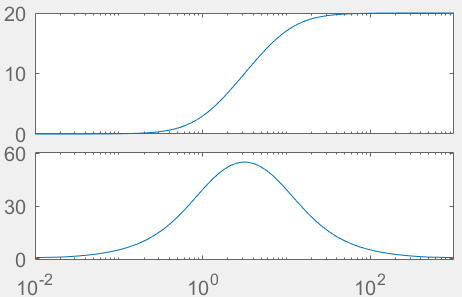
\includegraphics[width = \linewidth]{src/images/lead-controller.png}
    
    \titel{Lead-Controller}
        \begin{align*}
            0 < a < b
        \end{align*}
        improve command tracking/disturbance
rejection
– Pick $\frac{a}{b}$ as the desired increase in magnitude at low frequencies
– Multiply k by $\frac{a}{b}$ (this way the magnitude at high frequencies is unaffected).
– Pick a so that it is sufficiently smaller than
        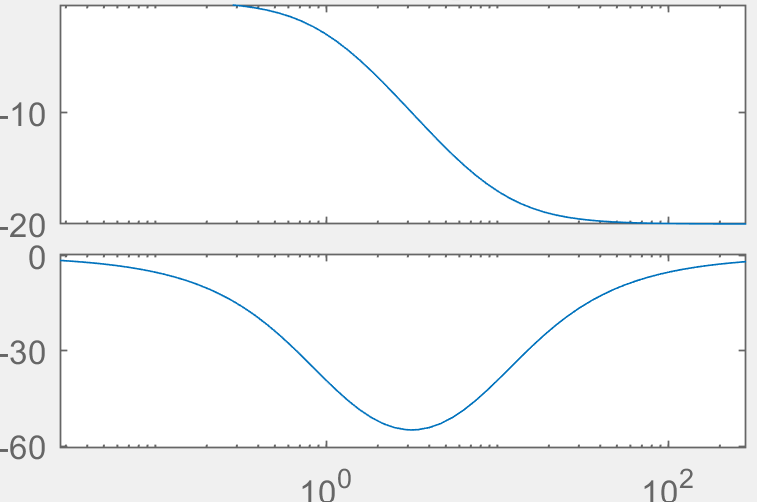
\includegraphics[width = \linewidth]{src/images/lag-controller.png}

    \titel{similarities of PID and Lead / Lag compensators}
        \begin{align*}
            PID(s) = k \cdot \underbrace{\frac{\frac{s}{z_1} + 1}{s + 0}}_{\text{Lag}} \cdot \underbrace{\frac{\frac{s}{z_2} + 1}{\frac{s}{p} + 1}}_{\text{Lead}}
        \end{align*}
        p refers to a "fast pole", This is necessary for the controller to be implementable